\section{Related Work}\label{relatedWork}
%Camera Path Animator 3.0 (Unity asset store).
%Camera system that follows the character but also focuses on showing the environment - Used in the game God of War.

During researching, a tool called Camera Path Animator 3.0 by Jasper Stocker was found \cite{unity_camTool}. It's can be used for creating animated cameras within Unity (see Figure \ref{fig:unity_path_cam_tool}). As the name suggests, it works by animating the camera along a specified path, which can have various shapes (e.g., Bezier and Hermite curves). The tool is primarily targeted towards creating cameras that move linearly along a set path, i.e. for use in a non-interative cutscene. It provides various ways of inserting, moving and deleting points, as well as settings that can be changed, such as field of view, speed, interpolation type and easing. Additionally, it has a event system for triggering certain events at certain points in the path.

\begin{figure}[htbp]
\centering
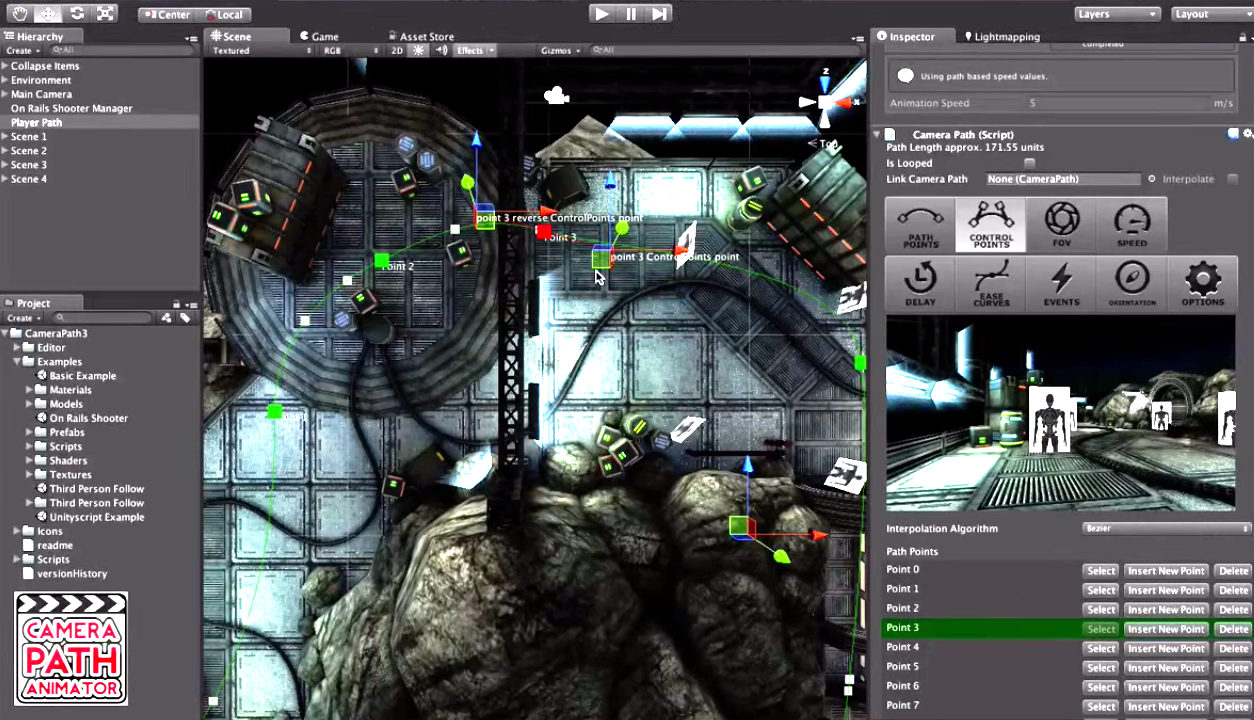
\includegraphics[width=0.50\textwidth]{Pics/unity_path_cam_tool}
\caption{Overview of the objects related to the camera system.}
\label{fig:unity_path_cam_tool}
\end{figure}

The God of War video game franchise for the PlayStation systems has also made notable use of their camera systems. The developers call the system Rail Driven Cameras and consists of a 'rail' that will be placed in the game world. A camera is keyed in both ends of the rail, and the camera will then animate between them as the protagonist moves along the rail. % Det her føles pølse, ikke meget at skrive om det og super unscientific